\documentclass[a4paper,12pt]{article}

\usepackage[utf8]{inputenc}
\usepackage{graphicx}
\usepackage{amsmath}
\usepackage[serbian]{babel}
\usepackage{url}
\usepackage[T1]{fontenc}
\usepackage{lmodern}

\usepackage{listings}
\usepackage{xcolor}

\lstset{
    language=Python,
    basicstyle=\ttfamily\small,
    keywordstyle=\color{blue},
    commentstyle=\color{gray}\itshape,
    stringstyle=\color{red},
    numbers=left,
    numberstyle=\tiny\color{gray},
    stepnumber=1,
    numbersep=5pt,
    showstringspaces=false,
    breaklines=true,
    frame=single,
}

\renewcommand{\figurename}{Slika}  % Change "Figure" to "Slika"
\renewcommand{\tablename}{Tabela}
\begin{document}

\begin{titlepage}
    \centering
	\begin{figure}[htbp]
    	\centering
    	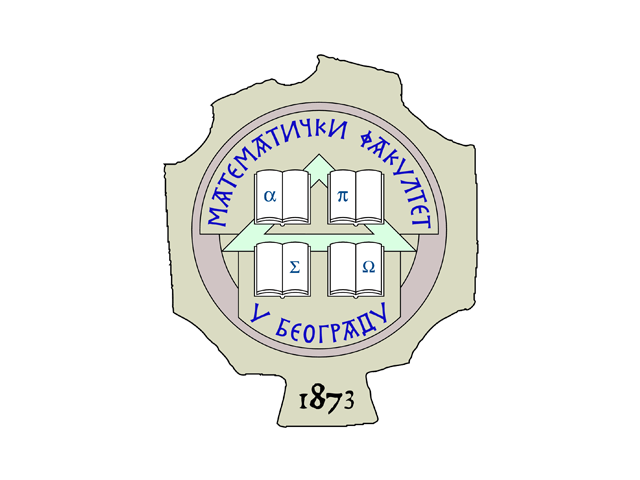
\includegraphics[width=0.4\textwidth]{images/logo.png}
	\end{figure}
    { Univerzitet u Beogradu \\ Matematički fakultet\par}
	
    \vfill

    {\Large \textbf{Seminarski rad}\par}

    \vspace{1cm}

    {\Large \textbf{Primena n-gramske analize na amino-kiselinske i nukleotidne kodove}\par}

    \vfill

    
	
	
	\begin{tabbing}
	\hspace{10cm} \= \hspace{10cm} \= \kill
	\textbf{Mentor:} \>  \textbf{Studenti:} \\
	Prof. dr Nenad Mitić \> Iva Milutinović 262/2021 \\
	Katedra za računarstvo i informatiku \> Jovana Urošević 189/2021 \\
	\> Smer: Informatika
	\end{tabbing}

    \vfill

    \textbf{Datum:} 2024/25

\end{titlepage}
\newpage
\tableofcontents
\newpage
\section{Uvod}
\newpage
\section{Parsiranje podataka i n-gramska analiza}
\textbf{Podaci i izvor:} U cilju klasterovanja i određivanja pravila pridruživanja više vrsta virusa (SARS-CoV-2, MERS, Ebola i Marburg), prikupljeni su sekvencioni podaci sa portala \textbf{NCBI Virus:} \url{https://www.ncbi.nlm.nih.gov/labs/virus/vssi/#/find-data/virus}. Primenjeni su filteri: \textit{ambiguous characters = 0} (isključivo
sekvence bez dvosmislenih simbola) i \textit{nucleotide completeness = complete} (samo kompletni genomi).

Zbog ogromnog broja dostupnih izolata, za SARS-CoV-2 korišćen je ograničen skup tačno određenih
\textit{accession} brojeva, dok su za ostale viruse preuzete sve dostupne kompletne sekvence koje ispunjavaju
zadate kriterijume. U nastavku su opisani koraci parsiranja i obrade podataka za proteinske (amino-
kiselinske) i nukleotidne FASTA fajlove, uključujući n-gramsku analizu i konstrukciju matrica frekvencija koje
su kasnije korišćene za klasterovanje i pravila pridruživanja.

\subsection{Parsiranje amino-kiselinskih FASTA fajlova}

\textbf{Format FASTA fajla:} Proteinske sekvence su preuzete u FASTA formatu, gde je svaka sekvenca
predstavljena zaglavljem i nizom jednoslovnih kodova aminokiselina. Zaglavlje počinje znakom \texttt{>} praćenim
opisom ili identifikatorom sekvence. U primeru FASTA zapisa ispod, zaglavlje sadrži jedinstveni identifikator i opis:

\begin{lstlisting}[language=]
>gi|5524211|gb|AAD44166.1| cytochrome b [Elephas maximus maximus]
LCLYTHIGRNIYYGSYLYSETWNTGIMLLLITMATAFMGYVLPWGQMSFW...
\end{lstlisting}

Ovaj primer ilustrije da zaglavlje često uključuje naziv proteina i naziv organizma u uglastim zagradama. U kontekstu naših podataka, naziv virusa (npr. Ebola virus, SARS-CoV-2) tipično je naveden u zagradama,
dok pre njega stoji naziv proteina (npr. spike glycoprotein, nucleocapsid protein). FASTA fajl može sadržati više
sekvenci (tzv. multi-FASTA format), jedna za drugom, gde svaki zapis počinje svojim \texttt{>} zaglavljem.

\vspace{10pt}
\textbf{Objedinjavanje podataka i mapiranje virusa/proteina:} Preuzete FASTA datoteke (odvojene
po virusima) parsirane su programskim putem i objedinjene u jedinstvenu
strukturu podataka radi dalje obrade. Svaki zapis u strukturi predstavlja jedan virusni protein i čuva sledeće
informacije: (i) identifikator ili naziv virusa, (ii) naziv/tip proteina, i (iii) aminokiselinsku sekvencu. Parsiranje
je ostvareno prolaskom kroz FASTA fajl liniju po liniju: kada se detektuje linija koja počinje sa \texttt{>} tretira se
kao zaglavlje, iz kojeg se ekstrahuju podaci o virusu i proteinu, dok se naredne linije pridružuju sekvenci
proteina. 

\vspace{10pt}
\textbf{Pseudokod za parsiranje FASTA fajlova:}

\begin{lstlisting}
for line in open("virus_proteins.fasta"):
    if line.startswith(">"):
        header = line[1:].strip()
        protein_name = header.split("[")[0].strip()
        virus_name = header.split("[")[1].rstrip("]")
    else:
        seq = line.strip() 
\end{lstlisting}

U gornjem primeru, string iz zaglavlja se deli na deo pre i posle znaka \texttt{[} kako bi se dobili naziv proteina i
naziv virusa. Tako svaki zapis povezujemo sa odgovarajućim virusom i proteinskim produktom. Mapiranje
virusa i proteina rešeno je tako što su nazivi virusa i proteina sačuvani kao posebna polja ili kao deo
jedinstvenog ključa. 

\vspace{10pt}
\textbf{Filtriranje dvosmislenih simbola:} Kako je navedeno, korišćene su sekvence bez neodređenih znakova
(\textit{ambiguous characters = 0}). Ipak, prilikom parsiranja je verifikovano da u amino-kiselinskim sekvencama
ima dvosmislenih kodova poput B, J, O, U, X, Z. Ovi znakovi predstavljaju ili ne-standardne ili neodređene
aminokiseline: npr. B označava asparagin ili asparaginsku kiselinu (Asx), Z glutamin ili glutaminsku kiselinu
(Glx), J leucin ili izoleucin (Xle), X bilo koju aminokiselinu (nepoznatu), dok su O i U specijalni kodovi za
nekanonske aminokiseline pirolizin i selenocistein. Sekvence koje bi sadržale takve simbole bile bi
filtrirane ili označene za izuzimanje kako bi se obezbedilo da analiza n-grame vrši samo nad 20 standardnih
aminokiselina. 

\subsection{N-gramska analiza proteinskih sekvenci}

Za svaku amino-kiselinsku sekvencu generisani su podnizovi
fiksne dužine (n-grami) i izračunate njihove učestalosti. Odabrane su dužine od 3, 4 i 5 (trigrami, tetragrami i
pentagrami) kako bi se uhvatili motivi u proteinskim sekvencama različitih veličina. N-gram analiza je
implementirana kliznim prozorom duž sekvence: za dati n , pomera se prozor od početka do kraja
sekvence i izdvaja svaki podniz dužine n . Broj mogućih različitih n-grama za aminokiselinske sekvence je
velik (maksimalno $20^n$ kombinacija za standardnih 20 aminokiselina), ali se u praksi javljaju samo
podskupovi te liste. Postupak za generisanje i brojanje n-grama po svakoj sekvenci može se opisati sledećim
koracima:

\begin{enumerate}
  \item \textbf{Generisanje n-grama:} za svaki indeks i u sekvenci od 1 do (L–n+1) uzima se podniz seq[i:i+n]
(dužine n). Na primer, za sekvencu "ACDEFGH" i n=3 dobili bismo trigrami: "ACD", "CDE", "DEF",
itd.
  \item \textbf{Brojanje učestalosti:} za svaku sekvencu se vodi rečnik (mapa) ili brojač pojavljivanja n-grama. Svaki
put kada se generiše n-gram, uveća se njegov brojač za tu sekvencu.
  \item \textbf{Skladištenje rezultata:} nakon prolaska kroz celu sekvencu, rezultujući brojači predstavljaju profil
sekvence u prostoru n-grama.
\end{enumerate}

\textbf{Primer generisanja trigram n-grama:}

\begin{lstlisting}
seq = "ACDEFGH"
n = 3
ngrams = [seq[i:i+n] for i in range(len(seq) - n + 1)]
# Rezultat: ["ACD", "CDE", "DEF", "EFG", "FGH"]
\end{lstlisting}

Slično tome, koristeći kolekciju Counter iz biblioteke collections, lako se dobiju frekvencije svakog n-grama
za sekvencu.

\vspace{10pt}
\textbf{Konstrukcija matrice frekvencija:} Nakon što su izračunate frekvencije n-grama za svaku proteinsku
sekvencu, podaci su organizovani u veliku matricu (tabelu), koja je zatim snimljena u CSV formatu radi lakše
analize. U toj matrici svaki red odgovara jednom proteinu (jednoj sekvenci) identifikovanom kombinacijom
virusa i naziva proteina, a svaka kolona odgovara jednom mogućem n-gramu dužine 3, 4 ili 5. Element
matrice $M_{ij}$ predstavlja broj pojavljivanja određenog n-grama j u proteinu i. Kolone su najpre
generisane unijom svih n-grama koji se uopšte pojavljuju u bilo kojoj sekvenci (za dati n), a za sekvence u
kojima neki motiv nije prisutan automatski će vrednost biti 0 u toj koloni. Tako su napravljene tri odvojene
matrice – za trigrame, tetragrame i pentagrame – s tim da svaka sadrži |V| redova (ukupan broj proteinskih
sekvenci svih posmatranih virusa) i $N_{n}$ kolona (broj različitih n-grama dužine n pronađenih u
celom skupu). Ove matrice predstavljaju kvantitativnu numeričku reprezentaciju proteinskih sekvenci,
pogodnu za primenu pravila pridruživanja i klasterovanja.

\subsection{Parsiranje nukleotidnih FASTA fajlova}

\textbf{Specifičnosti genomskih sekvenci:} Za analizu nukleotidnih sekvenci korišćeni su kompletni genomi virusa
iz iste grupe (SARS-CoV-2, MERS-coronavirus, različiti Ebolavirus i Marburgvirus). FASTA fajlovi za genome
sličnog su formata kao proteinski, ali zaglavlja obično sadrže naziv virusa i često sam \textit{accession} broj
bez posebnog naziva gena (jer je sekvenca čitav virusni genom). Na primer, zaglavlje može izgledati:

\begin{lstlisting}[language=]
>NC_002549 Marburg virus isolate Musoke, complete genome
\end{lstlisting}

Parsiranje ovih fajlova obavljeno
je slično kao za proteine – čitanjem svake linije i izdvajanjem meta-podataka iz zaglavlja. Iz svakog zaglavlja
izolovan je naziv virusa (npr. "Marburg virus", "Bombali ebolavirus", "SARS-CoV-2"), dok je cela naredna sekvenca (koja može imati i više hiljada nukleotida) sačuvana kao
string. U strukturi podataka, svaki zapis je predstavljao jedan genom, povezan sa svojim virusom (i
sojem), što omogućava da se kasnije rezultati grupišu po tipovima virusa.

\vspace{10pt}
\textbf{Filtriranje nevalidnih nukleotidnih simbola:} Kao i kod proteina, osigurano je da nukleotidne sekvence ne
sadrže dvosmislene kodove. Standardna nukleotidna abeceda obuhvata samo A, C, G, T (U), dok su ostala
slova deo IUPAC oznaka za neodređene baze. U takve spadaju: B, D, H, K, M, R, S, V, W, Y, N, koje
označavaju višestruke ili nepoznate nukleotide (npr. N znači bilo koja baza; R znači purina A/G; Y pirimidina
C/T; K = G/T, itd.). U procesiranju je urađena provera
te se svi nedozvoljeni simboli uklanjaju, jer bi u suprotnom narušili tačnost n-
gram analize (npr. podniz "ACNGA" ne može se smatrati validnim 5-merom zbog 'N').

\subsection{N-gramska analiza nukleotidnih sekvenci}

Za poređenje celih genoma, korišćena je analiza frekvencije
dužih n-grama dužine 6, 7, 8 i 9. Razlog za izbor ovih dužina je što kraći n-grami(poput
tri- ili pet-nukleotidnih) mogu biti manje informativni zbog kratkih ponavljajućih motiva i ograničene
kombinatorike ($4^3 = 64$
 mogućih trinukleotida), dok duži n-grami pružaju ekspresivniji "potpis"
genomske sekvence. Postupak generisanja 6–9-grama identičan je onome opisanom za proteine: za svaki
genom, prolazi se duž niza nukleotida i prave se svi podnizovi dužine n, nakon čega se broje pojavljivanja. Svaki genom dužine L sadržaće (L–n+1) n-grama dužine. Broj mogućih različitih n-grama
eksponencijalno raste sa n. Za DNA abecedu od 4 slova: \begin{itemize}
    \item $4^6 = 4096$ mogućih 6-mer podnizova
    \item $4^9 = 262144$ mogućih 9-mer podnizova
\end{itemize}
U
implementaciji, za svaki od izabranih n vrednosti generisana je posebna frekventna distribucija za dati
genom.

\vspace{10pt}
\textbf{Kreiranje matrica po virusima:} S obzirom da su genomske sekvence duže i da se skupovi sekvenci
razlikuju po virusima, frekvencije n-grama su inicijalno računane odvojeno za svaki virusni skup. Za svaki virus
(npr. za sve sekvence SARS-CoV-2, posebno za sve sekvence ebolavirusa itd.) formirana je matrica gde su
redovi pojedinačni genomski izolati tog virusa, a kolone predstavljaju n-gram frekvencije. U svaku matricu
uključeni su svi n-grami dužine n koji su se pojavili u barem jednom genomu posmatranog virusa, pri čemu
su za sekvence koje ih ne sadrže vrednosti 0. Nakon što su generisane takve matrice za svaki virus posebno,
one su po potrebi spojene zajedno kako bi se omogućilo poređenje između različitih virusa.
Sličan pristup sačuvan je kao kod proteina: izrađene su posebne matrice za 6-mer, 7-mer, 8-mer i 9-mer
analize. Svaka matrica ima onoliko redova koliko je genoma uzeto u obzir za dati virus, a kolona onoliko
koliko ima različitih n-grama te dužine u celom skupu. Ove CSV matrice predstavljaju kvantitativne
karakteristike genoma i čine osnovu za dalju analizu sličnosti sekvenci.


\newpage
\section{Klasterovanje}

\subsection{SOM (Self-Organizing Map)}
\textbf{SOM (Self-Organizing Map)} ili samoorganizujuća mapa je algoritam neuronskih mreža koji koristi neurone bez nadzora (unsupervised learning) kako bi izvršio projekciju visokodimenzionalnih podataka u dvodimenzionalni prostor, uz očuvanje topoloških relacija između ulaznih podataka.

Glavna prednost SOM-a jeste što ne zahteva prethodno definisane klase, već sam organizuje podatke na osnovu njihove sličnosti i strukture.

SOM mapira slične ulazne vektore na bliske pozicije na mreži neurona (najčešće 2D mreža), čime omogućava vizualnu i analitičku interpretaciju klastera. Tipično se koristi u bioinformatici, prepoznavanju obrazaca, genomskoj klasifikaciji, vizuelizaciji kompleksnih podataka i detekciji anomalija.

\textbf{Način funkcionisanja Self-Organizing Map algoritma:}SOM se sastoji od dvodimenzionalne mreže neurona, gde svaki neuron ima svoj vektor težina iste dimenzije kao ulazni podaci. Algoritam prolazi kroz sledeće korake:

\begin{enumerate}
  \item \textbf{Inicijalizacija težina:} Nasumično ili linearnom interpolacijom.
  \item \textbf{Poređenje:} Za svaki ulazni vektor određuje se neuron čiji je vektor težina najsličniji ulazu (tzv. BMU – Best Matching Unit).
  \item \textbf{Ažuriranje težina:} Težine BMU-a i njegovih suseda u mreži se ažuriraju tako da se približe ulaznom vektoru. Promene su kontrolisane koeficijentom učenja i funkcijom susedstva.
  \item \textbf{Iteracija:} Postupak se ponavlja za sve ulazne vektore i tokom više epoha. Tokom vremena se smanjuju koeficijent učenja i širina susedstva.
\end{enumerate}

\textbf{Primena SOM-a u kontekstu naše analize:} U analizi viralnih sekvenci, radimo sa vektorima visokih dimenzija koji predstavljaju frekvencije n-grama u genomskim i proteinskim sekvencama. Takvi vektori nisu lako interpretabilni niti vizuelizovani u 2D prostoru. SOM je idealan za ovaj zadatak iz nekoliko razloga:
\begin{itemize}
    \item Preslikava složene podatke u 2D prostor, što omogućava jednostavnu vizualizaciju.
    \item Zadržava sličnost – sekvence sa sličnim n-gram profilima biće mapirane u blizini.
    \item Ne zahteva unapred poznat broj klasa ili oznake (klasteruje bez nadzora).
    \item Omogućava detekciju grupacija među sekvencama različitih virusa i proteina.
\end{itemize}

\textbf{Parametri SOM algoritma koje smo koristile:}
\begin{itemize}
    \item Dimenzije mreže(som\_x, som\_y): 15x15 neurona(225 neurona u mreži)
    \item Broj iteracija: 1000 (broj epoha treniranja)
    \item Funkcija udaljenosti: Euklidska distanca
    \item Koeficijent učenja: 0.5
    \item Širina susedstva (sigma): 1.0
\end{itemize}

Ovi parametri su podešeni tako da omoguće postepenu konvergenciju mreže ka stabilnim klasterima i jasnu topološku strukturu među sekvencama.

\vspace{10pt}
\textbf{SOM nad amino-kiselinskim sekvencama}
\vspace{10pt}

Kod amino-kiselinskih sekvenci koristile smo već prethodno generisane n-gram matrice (n = 3, 4, 5), gde je svaka sekvenca predstavljena kao vektor frekvencija n-grama. Ove matrice su sadržavale i dodatne kolone sa oznakama:

\begin{itemize}
    \item virus\_type – oznaka virusa (npr. SARS-CoV-2, Marburg virus)
    \item protein\_type – oznaka proteina (npr. GP, spike, E protein)
\end{itemize}

Kako bismo istražile strukturu podataka, SOM algoritam je pokrenut dva puta:
\begin{enumerate}
  \item \textbf{Grupisanje prema tipu virusa}
  \item \textbf{Grupisanje prema tipu proteina} 
\end{enumerate}

U oba slučaja, oznake (`virus\_type` ili `protein\_type`) nisu korišćene u učenju mreže, već samo u bojenju rezultata, kako bismo proverile da li SOM klasteri odgovaraju biološkim kategorijama.

Podaci su standardizovani pomoću StandardScaler() – čime su sve vrednosti vektora n-gram frekvencija skalirane na istu skalu (normalizovane), što je ključno za stabilan rad SOM algoritma.

\textbf{Vizualizacije i interpretacija:}
Koristile smo dve vrste vizualizacija za svaku n-gram kombinaciju:
\begin{enumerate}
  \item \textbf{U-Matrix (distance map):} Prikazuje razdaljine između susednih neurona na mapi. Tamnije oblasti predstavljaju veće razlike između susednih neurona i ukazuju na granične linije između klastera.
  \item \textbf{Mapa neurona sa tačkama:} Sekvence su predstavljene tačkama, mapirane na pozicije njihovih BMU neurona i obojene prema tipu virusa ili proteina.
\end{enumerate}

\begin{figure}[h!]
    \centering
    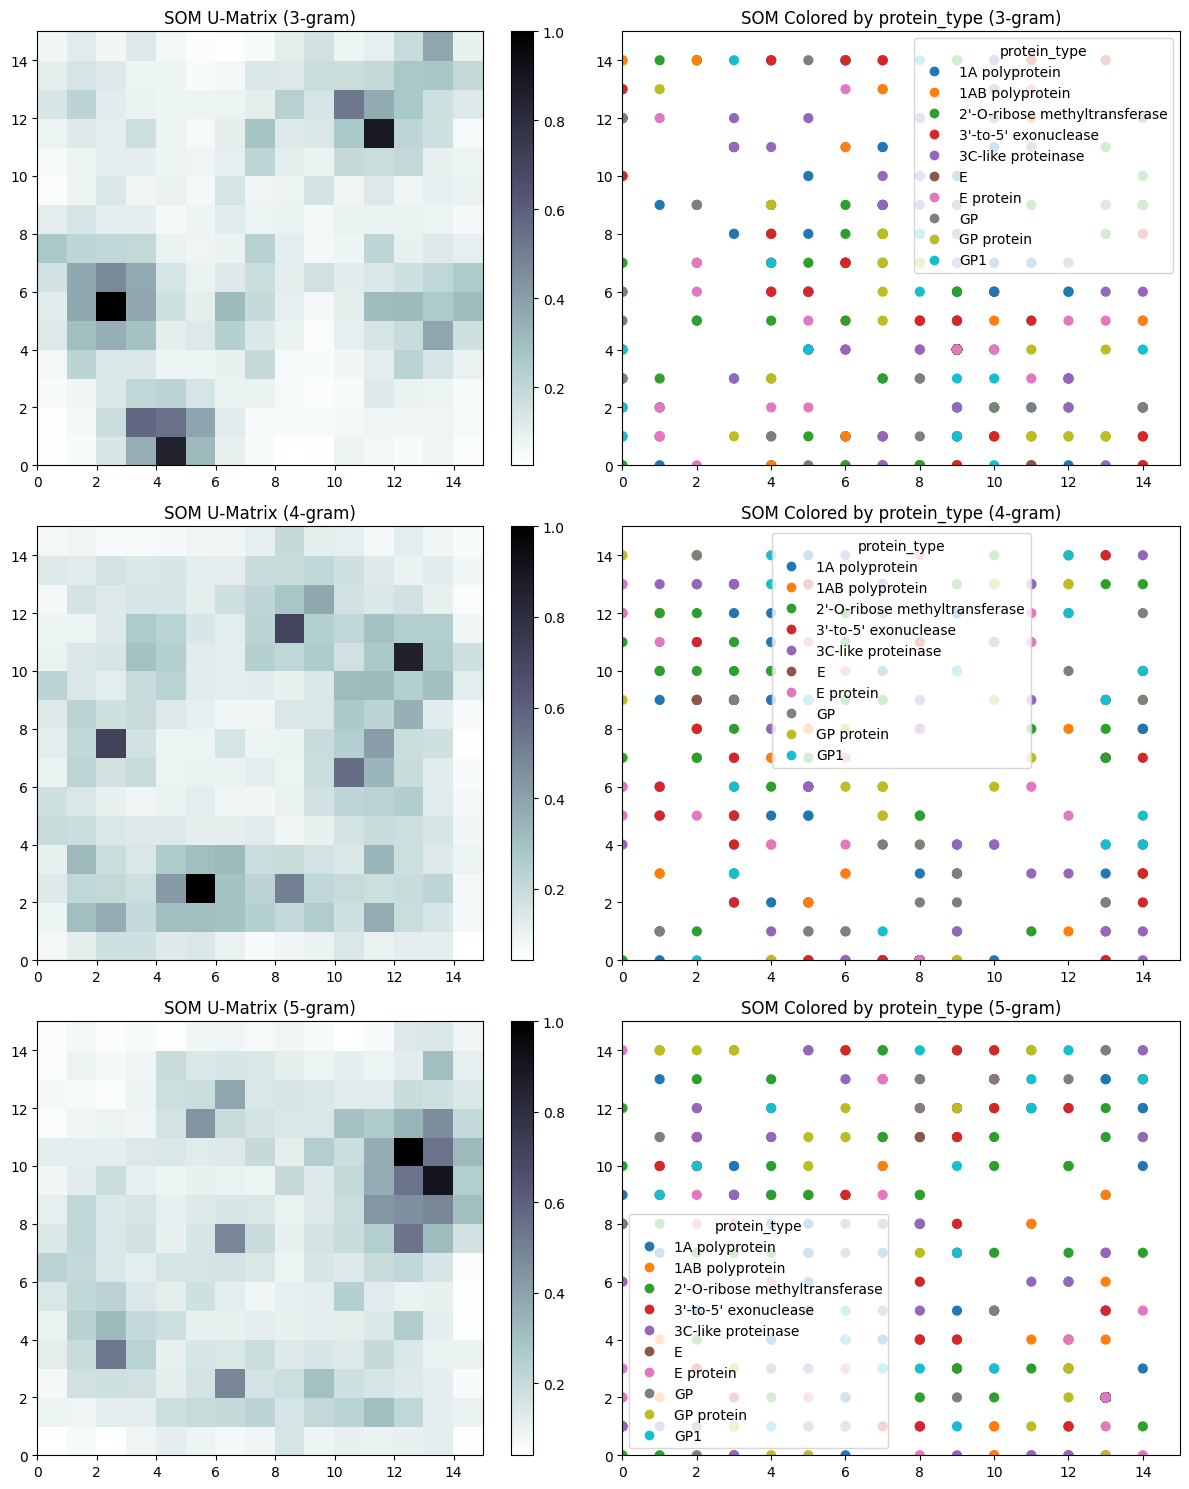
\includegraphics[width=0.5\textwidth]{images/som-amino-acid-protein.png}
    \caption{Vizualizacija za grupisanje prema tipu proteina}
    \label{fig:som-struktura}
\end{figure}

\textbf{Diskusija rezultata:}
SOM mreža identifikovala je veliki broj klastera (132–171), što ukazuje na visoku raznovrsnost sekvenci i izražene razlike u n-gram profilima između različitih virusa i proteina. Neke ključne opservacije:

\begin{itemize}
    \item Povećanjem n-gram dužine sa 3 na 5, broj klastera raste – to je očekivano jer duži n-grami bolje diferenciraju sekvence, ali istovremeno povećavaju sparsenost podataka.
    \item Klasteri se često grupišu po tipu virusa – što pokazuje da sekvence virusa istog tipa imaju slične n-gram profile.
    \item Grupisanje po tipu proteina otkriva klastere gde različiti virusi proizvode funkcionalno slične proteine – npr. spike proteini iz različitih koronavirusa su često blizu na mapi.
\end{itemize}

Broj BMU klastera koji su različiti (tj. unikatne pozicije na SOM mapi koje su bile aktivne) predstavlja broj funkcionalno različitih grupa koje je mreža detektovala. Veći broj klastera može ukazivati i na visoku rezoluciju mreže, ali i na kompleksnost podataka.

\begin{figure}[h!]
    \centering
    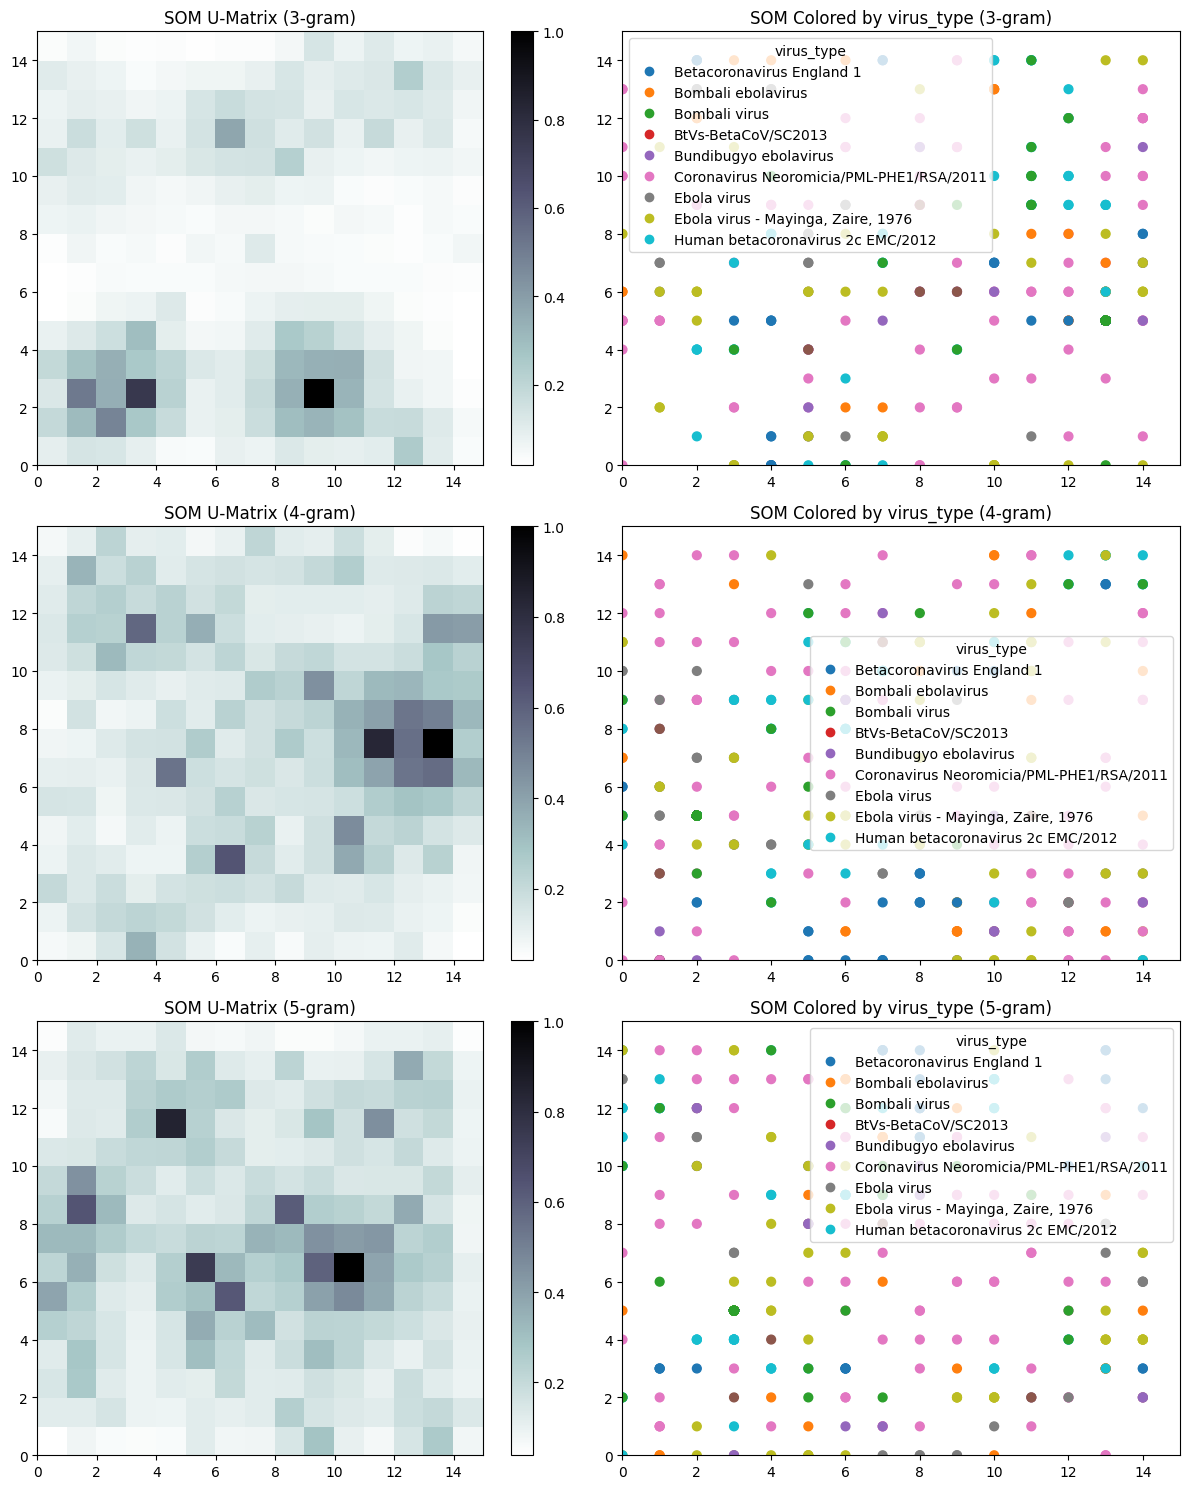
\includegraphics[width=0.5\textwidth]{images/som-amino-acid-virus.png}
    \caption{Vizualizacija za grupisanje prema tipu virusa}
    \label{fig:som-struktura}
\end{figure}

\textbf{Slika 1 i 2:} Primer rezultata samoorganizujuće mape za proteinske sekvence (3-gram frekvencije
aminokiselina). Prikazana je U-matrica SOM mreže, gde tamnija boja označava veće rastojanje između
neurona (granične oblasti klastera). Preko toga je izvršeno bojenje po vrsti virusa čiji protein pripada
datom neuronu. Vidljivo je grupisanje proteina istog virusa u zajedničke klastere (npr. proteini ebolavirusa
grupisani zajedno, odvojeni od koronavirusnih proteina), što ukazuje da i prostori 3-grama nose filogenetski
signal za razlikovanje virusa. Slični rezultati dobijeni su i za 4-gram i 5-gram frekvencije, što dodatno potvrđuje stabilnost ovog pristupa. Na tamnijim mestima SOM mape primećuje se nedostatak sekvenci, dok je u drugim delovima jasno uočljivo kako su klasteri međusobno razdvojeni.

\vspace{20pt}
\textbf{SOM nad nukleotidnim sekvencama}
\vspace{10pt}

Za nukleotidne sekvence korišćene su n-gram matrice za dužine 6, 7, 8 i 9, izgrađene na osnovu kompletnih genoma virusa. Svaki red u matrici predstavlja jedan genom (izolat), dok su kolone različiti n-grami. Pošto se ovde radi o dužim sekvencama sa više stabilnih obrazaca, korišćeni su i duži n-grami nego kod proteina. Oznaka `virus\_type` se koristila kao labela za bojenje tačaka.

\vspace{10pt}
\textbf{Vizualizacije i interpretacija:}
Koristile smo iste dve vizualizacije:
\begin{enumerate}
  \item \textbf{U-Matrix (distance map):} Za identifikaciju granica između klastera.
  \item \textbf{Mapa neurona sa tačkama:} Svaka sekvenca je prikazana kao tačka, bojena prema virusu (npr. SARS-CoV-2, Ebola virus), čime se uočava grupisanje genoma po virusnim vrstama.
\end{enumerate}

\textbf{Diskusija rezultata:}
Za razliku od amino-kiselinskih podataka, SOM mreža je za sve nukleotidne n-grame proizvela konzistentan broj od 28 klastera. Ovaj broj veoma verovatno odgovara broju različitih virusnih izolata ili grupacija, što ukazuje da:

\begin{itemize}
    \item Genomske sekvence su znatno homogenije unutar iste vrste, ali dovoljno različite među vrstama da ih SOM može jasno razdvojiti.
    \item SOM je detektovao jasne evolutivne i taksonomske granice između genoma virusa (npr. između ebolavirusa i koronavirusa).
    \item Za razliku od proteinskih sekvenci koje imaju veću unutrašnju raznovrsnost (različiti proteini jednog virusa), kompletni genomi se ponašaju kao stabilniji entiteti, pa su i rezultati klasterovanja stabilniji.
\end{itemize}

\begin{figure}[h!]
    \centering
    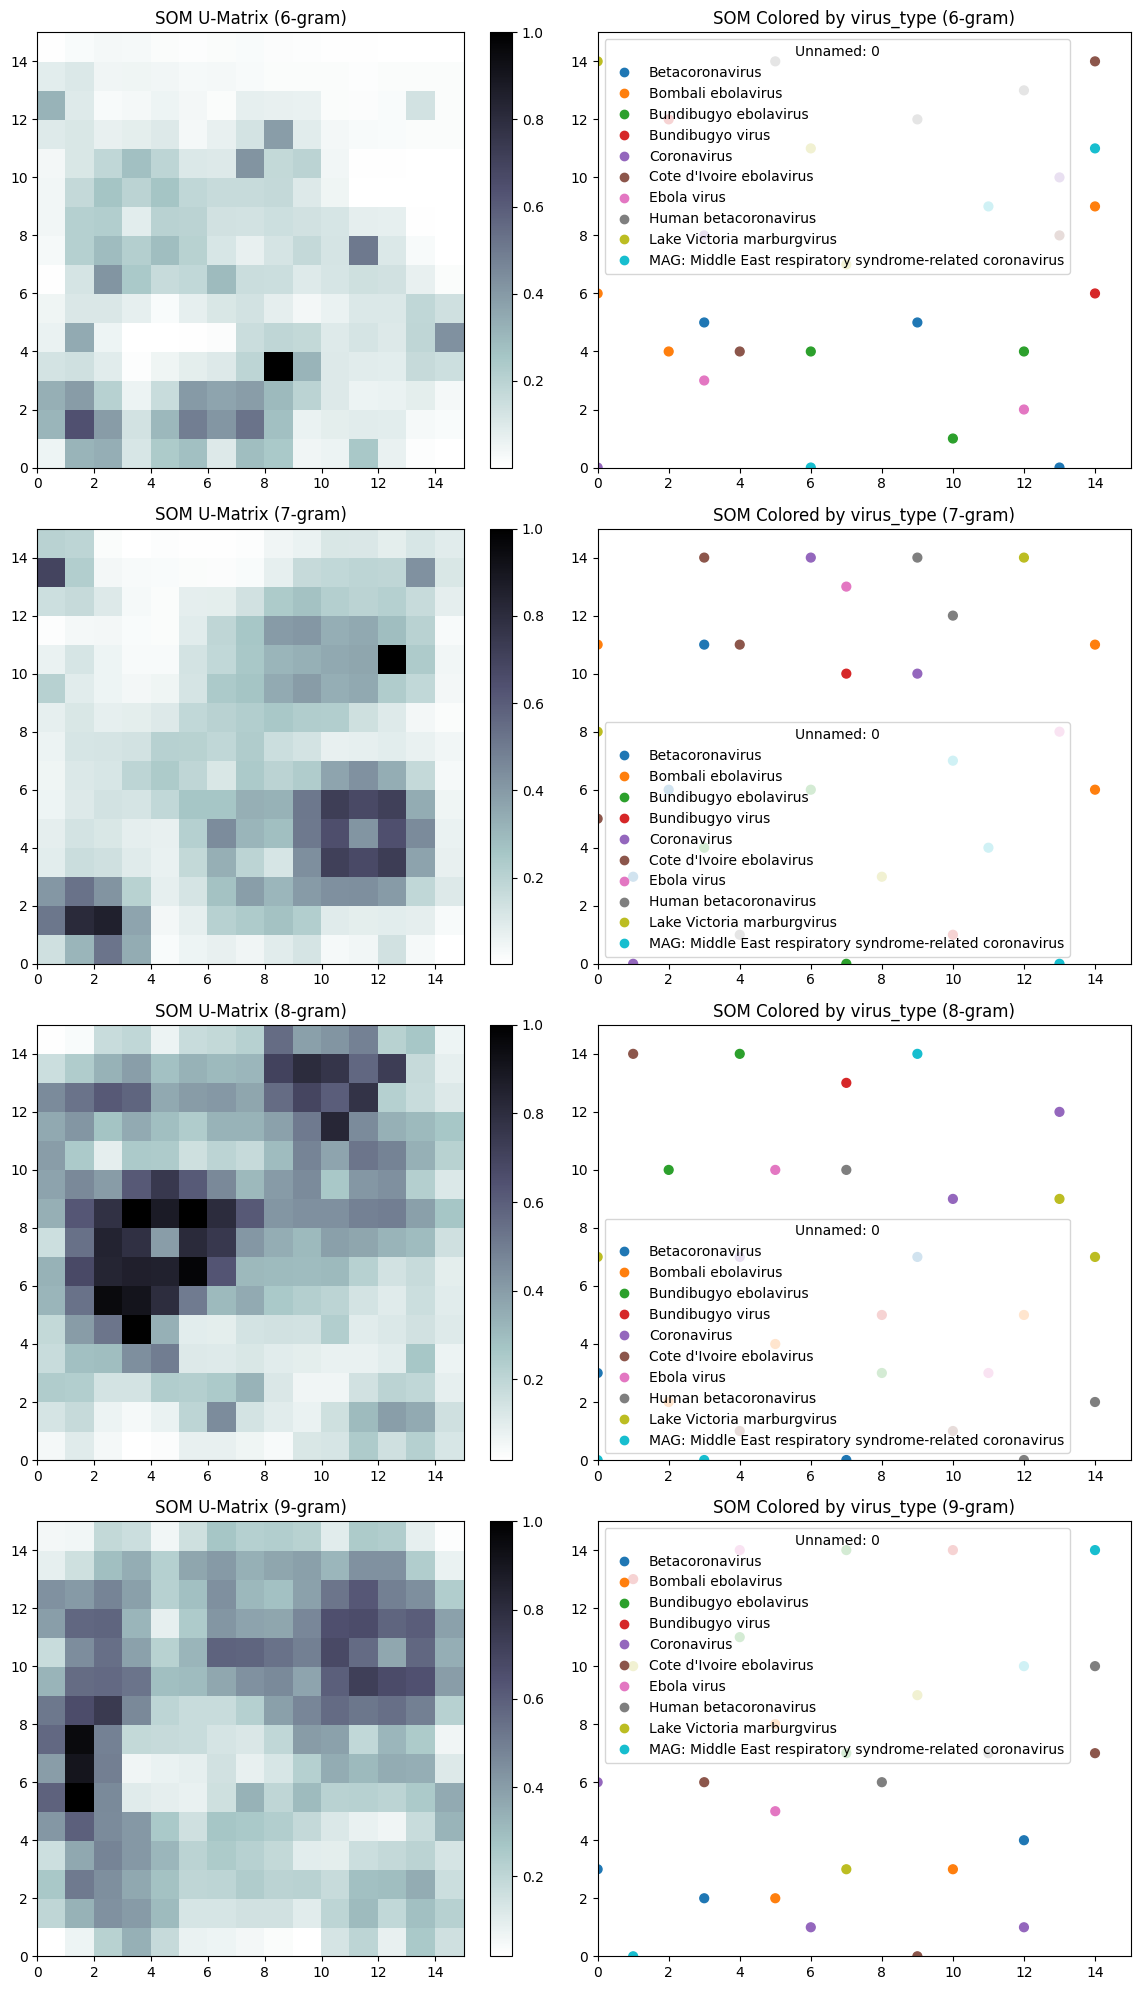
\includegraphics[width=0.5\textwidth]{images/nucleotide-virus.png}
    \caption{Vizualizacija za grupisanje prema tipu virusa}
    \label{fig:som-struktura}
\end{figure}

\textbf{Slika 3:} Primer rezultata za nukleotidne sekvence – SOM projekcija na osnovu 6-mer frekvencijskih profila
kompletnog genoma. Svaka tačka predstavlja jedan virusni genom, obojen prema tipu virusa (legenda
desno: različite boje za SARS-CoV-2, MERS, različite vrste ebolavirusa i marburgvirusa). Uočljivo je grupisanje
genoma iste virusne vrste u kompaktnije klastere. Na primer, genomi ebolavirusa (različitih sojeva/species)
mapirani su blizu jedni drugih (zelene nijanse), dok su koronavirusi (plave nijanse) razdvojeni u drugi deo
mape. Ovakvi rezultati potvrđuju da matrice n-gram frekvencija, konstruisane opisanim postupkom
parsiranja i obrade podataka, predstavljaju dobru osnovu za primenu SOM algoritma i efikasno
klasterovanje viralnih sekvenci. Kao i za 6-grame, i kod 7-grama, 8-grama i 9-grama uočavaju se izraženija razdvajanja i jasnije formirani klasteri, ali se sa porastom broja n ujedno šire i prazni delovi mape, što ukazuje na sve ređu pokrivenost prostora sekvencama.

\vspace{200pt}
\textbf{Zaključak:}

\vspace{10pt}
\textbf{SOM algoritam} se pokazao kao efikasan i interpretabilan metod za nadozorovano klasterovanje kako proteinskih, tako i genetskih sekvenci. Njegova sposobnost da projektuje podatke u 2D prostor i da očuva topološku strukturu omogućila nam je da:

\begin{itemize}
    \item Identifikujemo grupe sličnih sekvenci prema tipu virusa i tipu proteina.
    \item Uočimo evolutivno povezane sekvence, čak i između različitih virusa.
    \item Potvrdimo da n-gramski profil predstavlja pouzdanu reprezentaciju za bioinformatičko klasterovanje.
\end{itemize}

\newpage

%\begin{thebibliography}
    
%\end{thebibliography}

\end{document}
